\documentclass[11pt,a4paper]{article}
\usepackage{enumitem,amssymb,graphicx,epstopdf,hyperref,authblk,minted,expl3,listings}
\usepackage[T1]{fontenc}
\usepackage[utf8]{inputenc}
\usepackage[lmargin=2.5cm, rmargin=2.5cm,tmargin=3cm,bmargin=2.5cm]{geometry}

\begin{document}

\title{Introduction to Micro-controllers}
\date{\today} 
\author{Andres LaRosa}
\author{Bret Comnes}
\affil{Portland State University}
\maketitle

\section{Introduction} % (fold)
\label{sec:introduction}

Microcontrollers are small computers designed to go where desktop computers dare not go.  They come in all shapes, sizes, and layouts.  Usually, they are quite small and use less power than traditional computers.  Microcontrollers are often deployed in an `appliances' and serve an unmodifiable dedicated purpose, such as keeping track of what spin cycle your washing machine is on, or how much time is left before it should turn off your microwave oven.  Make no mistake however, these are general purpose computers.  The other major difference between a microcontroller and traditional computers is that they they come with an array of analog and digital input and outputs. These can be used to read environmental data from sensors, talk to other computers or devices and electronically control other systems which provide environmental outputs such as a LCD screen, mechanical switch or servo motor etc.  \cite{wpmicro}

Getting started with microcontrollers can be tedious process, as they can require a number of supporting circuits, USB controllers, programmers, boot loaders, power supplies and chips, just to load your first program onto the microcontroller chip.  Often times you will start with a prototyping board, which takes a microcontroller and all the necessary tools to start working with it, and puts it on a single board, ready to start playing around with.

\subsection{Arduino} % (fold)
\label{sub:arduino}

\begin{figure}[htbp]
	\centering
		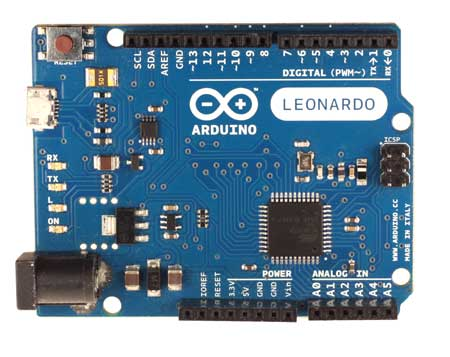
\includegraphics[height=2.7in]{figures/ArduinoLeonardoFront_2_450px.jpg}
	\caption{Arduino Leonardo\cite{leonardo}}
	\label{fig:figures_ArduinoLeonardoFront_2_450px}
\end{figure}


\begin{quote}
\emph{``Arduino is a tool for making computers that can sense and control more of the physical world than your desktop computer. It's an open-source physical computing platform based on a simple microcontroller board, and a development environment for writing software for the board.''} -- Arduino Website\cite{arduino-guide}
\end{quote}

This lab will be using the Arduino Leonardo Microcontroller\cite{leonardo}.  It is similar to the Arduino Uno\cite{uno}, with the major difference being that it uses SMT\cite{smt} instead of the older ``thru-hole''\cite{th} technology in order to reduce cost.

Arduino drastically lowers the difficulty of getting started with a microcontroller (compared to to plain ATMEGA/PIC/ARM chips), as it provides all the necessary tools to start making the microcontroller do interesting things without nearly all the setup of just a plain microcontroller.

Arduino is based around an 8-bit Atmel AVR microcontroller, and other good things like a boot loader for uploading programs, a USB controller for an easy source of power and connectivity to your computer as well as a barrel jack for non usb power sources.

It is programmed using a language that is based off of C++ and uses a fork of the Processing IDE used for writing, compiling and uploading your programs to the board.  Many Arduino projects you will find will rely on programs running on your computer using Processing, but it is not limited to this.\cite{processing}

% subsection arduino (end)

% section introduction (end)


\section{Getting Started} % (fold)
\label{sec:getting_started}

\subsection{Setting up your software} % (fold)

This lab is based off of the Arduino 1.0.3 software which can be downloaded for free from\cite{arduino-dl}.  Unlike other embedded systems development environments, the Arduino software is quick to download and set up, and has zero cost associated with the software which makes it a convenient to work with when your primary goal is to come up with a working prototype.

\subsection{Find a Computer} % (fold)
\label{sub:find_a_computer}
You are free to use your own laptop or one of the classroom computers.

% subsection find_a_computer (end)

\subsection{Download and Launch the Arduino Software} % (fold)
\label{sub:download_and_launch_the_arduino_software}
Visit \url{http://arduino.cc/en/Main/Software} and downloaded the latest Arduino software\cite{arduino-dl}.  If you have decided to use your own Arduino, make sure you find the necessary USB drivers if you have a board that is older than the Uno.

% subsection download_and_launch_the_arduino_software (end)

\subsection{Selecting the Board} % (fold)
\label{sub:selecting_the_board}
Once the IDE is open, navigate to the toolbar and select the board you are working with from \textbf{Toolbar $\rightarrow$ Tools $\rightarrow$ Board $\rightarrow$ Arduino Leonardo}.  Select a different board if you are using one.

% subsection selecting_the_board (end)

\subsection{Selecting a Serial Port} % (fold)

\label{sub:selecting_a_serial_port}
This step varies from system to system.  In this step, we tell the computer which serial port that the Arduino chip can be reached at, for programing the board, as well as talking to it during runtime.
    \begin{figure}[htbp]
        \centering
            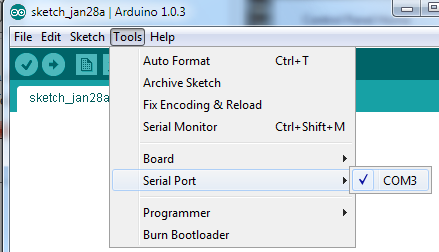
\includegraphics[height=2in]{figures/port-windows.png}
            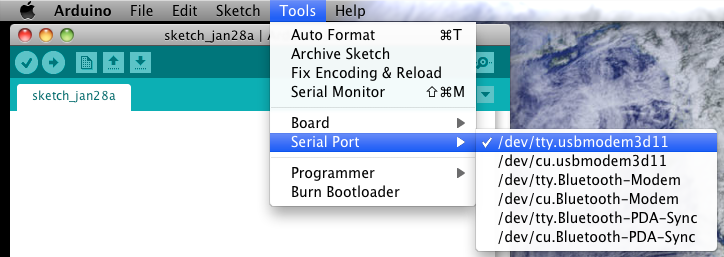
\includegraphics[height=1.5in]{figures/port-osx.png}
        \caption{Port Selection in Windows and OS X}
        \label{fig:figures_port}
    \end{figure}

\subsubsection{Windows} % (fold)

\label{ssub:windows}
Select \textbf{Toolbar $\rightarrow$ Tools $\rightarrow$ Serial Port $\rightarrow$ COM3} where COM3 is the serial port that has been assigned to your Arduino by windows.  You should only have one port available.

% subsubsection windows (end)

\subsubsection{OS X} % (fold)
\label{ssub:os_x}
Select \textbf{Toolbar $\rightarrow$ Tools $\rightarrow$ Serial Port $\rightarrow$ /dev/tty.usbmodem3d11} where COM3 is the serial port that has been assigned to your Arduino by windows.  You should only have one port available.

% subsubsection os_x (end)

% subsection selecting_a_serial_port (end)

\subsection{Uploading your first program} % (fold)
\label{sub:uploading_your_first_program}
Next we will open an example program, verify that it compiles, then upload it to our board.


Navigate to \textbf{Toolbar $\rightarrow$ File $\rightarrow$ Examples $\rightarrow$ 01. Basics $\rightarrow$ Blink}.  Press the verify button.  It should compile the sketch and return a `Done compiling' message.  If you get an error, something went wrong.

    \begin{figure}[htbp]
        \centering
            
\includegraphics{figures/verify.png}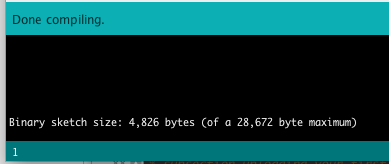
\includegraphics{figures/compile.png}
        \caption{Verify Button (Left) Compile Success Message (Right)}
        \label{fig:figures_verify}
    \end{figure}

    If that completed, go ahead and upload the program to the board by pressing the upload button (the button right next to verify button) and it should provide a similar completion message after a few moments.  The LEDs on the Arduino will blink during the upload, but should settle down after a few seconds.  Once the program you uploaded is running, the LED labeled `L' should be slowly blinking.  This LED labeled `L' is wired to Pin 13 on the Arduino, a digital pin with a resistor built in that so that LEDs can be added easily.  \textbf{Go ahead and add an LED between Pin 13 and GND}.  It should blink at the same rate as the `L' LED on the board.

% subsection uploading_your_first_program (end)


Congratulations!  You now have a working Arduino that is talking to the Arduino IDE.

% subsection setting_up_your_software (end)

% section getting_started (end)

\section{Programming Arduino} % (fold)
\label{sec:programming_arduino}

Arduino is based off the Processing\cite{processing} programming language, and has some similarities to C, however much of the language has been simplified.  In this section we will go over the basics of the language, look at some simple examples of code and even write some of our own.

\subsection{The Bare Minimum} % (fold)
\label{sub:the_bare_minimum}

The bare minimum code you need for an Arduino program can be seen in Figure~\ref{fig:bare}.

\begin{figure}[htbp]
	\centering
\begin{minted}[mathescape,
				linenos,
				numbersep=5pt,
				gobble=0,
				frame=lines,
				framesep=2mm]{c}
void setup() {
// put your setup code here, to run once:
}
void loop() {
// put your main code here, to run repeatedly: 
}
\end{minted}
	\caption{The minimum Amount of code for an Arduino Program}
	\label{fig:bare}
\end{figure}

There are two parts to this minimum program, the \texttt{void setup() \{\}} section and the \texttt{void loop() \{\}} section.  When your program runs, It starts executing your code, line by line, starting in the \texttt{void setup()} section, inside the brackets, \texttt{\{\}}, that follow.  Your program will execute any code that is in this section, and when it gets to the end, will begin executing the code inside \texttt{void loop() \{\}}, until it gets to the end of the available instructions, at which point, the program starts back over in at the beginning of \texttt{void loop() \{\}}, retaining any variables or settings from prior loops.

Lets look at a simple example, that you should already have pulled up, the \texttt{Blink} program, which is found in Figure~\ref{fig:blink}.  If you still need to open this, refer to Section~\ref{sub:uploading_your_first_program}.

% subsection the_bare_minimum (end)


\section{Understanding the Blink Program} % (fold)
\label{sec:understanding_the_blink_program}

\begin{figure}[htbp]
	\centering
\begin{minted}[mathescape,
				linenos,
				numbersep=5pt,
				gobble=0,
				frame=lines,
				framesep=2mm]{c}
/*
  Blink
  Turns on an LED on for one second, then off for one second, repeatedly.
 
  This example code is in the public domain.
 */
 
// Pin 13 has an LED connected on most Arduino boards.
// give it a name:
int led = 13;

// the setup routine runs once when you press reset:
void setup() {                
  // initialize the digital pin as an output.
  pinMode(led, OUTPUT);     
}

// the loop routine runs over and over again forever:
void loop() {
  digitalWrite(led, HIGH);   // turn the LED on (HIGH is the voltage level)
  delay(1000);               // wait for a second
  digitalWrite(led, LOW);    // turn the LED off by making the voltage LOW
  delay(1000);               // wait for a second
}
\end{minted}
	\caption{The Blink Program in all its glory}
	\label{fig:blink}
\end{figure}

If a block of text is wrapped in \texttt{/* */}, such as lines 1 thru 6 in Figure~\ref{fig:blink} or has a \texttt{//} in front of it on one line, such as line 12, means its a comment.  Comments are little notes you leave in your code, and are not executed or interpreted by your program in any way.  It is good practice to add comments to your code.  They can help you think about your program, and will also remind you, and others that see your code, what the program does or how it works.


Running down lines 1-9, we see that this is all comments describing the function of the program, how it works, and its license.   The first piece of code we see is on line 10.


\subsection{Variables} % (fold)
\label{sub:variables}

\mint{c}|int led = 13;|

The first thing to notice, is that this code is not inside \texttt{void setup()} or \texttt{void loop()}.  That is because it is a variable. 


Variables are an incredibly useful tool in any programming.  For the sake of simplicity, we will consider variables as a name that we decide upon, and that they are associated with a value.  This value could be the name of a pin on the Arduino.  It could be a number that we are storing for later, or it could be a message made up of a string of characters that we plan on displaying on an LCD screen. 

Any variable we decide to use, we have to describe to our program.  This is referred to as declaring your variable.  \textbf{Variables are declared before your \texttt{void setup()} or \texttt{void loop()} sections.}  Line 10 declares a variable named \texttt{led}, gives it a variable type of \texttt{int}, for integer, and then assigns it a value of 13.  This variable is used to reference the physical pin we will be using in our program.  It is used as an abstraction layer, so that if we ever go back and change which pin we want to use, we can update all the places in our program that reference this pin number simply by updating the initial variable value.

The basic syntax of a variable declaration is: 

\mint{c}|type variable_name = value;|

There are various variable types that you will be introduced through these tutorials.  Once the variable is declared, you can reference it in as many different parts of your program.  You can have your program change the value of the variable as a means to pass messages to other parts of your program.

% subsection variables (end) 

\subsection{Pin Modes} % (fold)
\label{sub:pin_modes}

After the variables (in this case, only one variable) are declared, the next piece of code we arrive at is our \texttt{void setup()}.  Stepping inside the curly braces of this structure, we come to the following line:

\mint{c}|pinMode(led, OUTPUT);|

The vast majority of programs on your Arduino will require that you have inputs and outputs to other components around your board.  There are a variety of pins on the Arduino that can do different things, like read voltages, generate digital signals, and produce PWM analog output voltages.  

Before you can use a pin in your program, you must tell your program how you will be using it.  It is similar the requirement of declaring a variable before you can use it.  

Here is the pin setup syntax.

\mint{c}|pinMode([PIN-NUMBER], [PIN-TYPE]);|

In the \textbf{Blink} code, we designate the pin associated with the \texttt{led} variable, pin 13, as an \texttt{OUTPUT}.  The \texttt{OUTPUT} type means that the pin is a digital pin that will output 0V or 5V, depending if we write \texttt{HIGH} or \texttt{LOW} to that pin in our program.

Each pin has a name assigned to it.  Each pin on the Arduino has its name printed next to it, which can be seen in Figure~\ref{fig:figures_ArduinoLeonardoFront_2_450px}.  A list of pins, and some of their useful possible pin types can seen in Table~\ref{tab:pintypes}~.  There are two types of input and output pins.  Digital and Analog pins.

Digital pins and read digital signals, and generate digital signals as well as PWM analog signals.  PWM, or Pulse Width Modulation, is a way to simulate analog voltage signals with a digital pin.  PWM capable pins have a ~ printed next to their name on the board.

Analog Pins can read in analog voltages between 0v and 5v and converts them to a value that your program can use between 0 and 1023.

\begin{table}[hct!]
\caption{Placeholder Table of Pins and output modes}
\label{tab:pintypes}
\centering
\begin{tabular}{cc|cc}
\hline \hline 
r1c1 & r1c2 & r1c3 & r1c4\\
\hline
r2c1 & r2c2 & r2c3 & r2c4\\
\hline
r3c1 & r3c2 & r3c3 & r3c4\\
\hline
r4c1 & r4c2 & r4c3 & r4c4\\
\hline
r5c1 & r5c2 & r5c3 & r5c4\\
\hline
r6c1 & r6c2 & r6c3 & r6c4\\
\hline \hline 
\end{tabular}
\end{table}

% subsection pin_modes (end)

\subsection{Generating Output} % (fold)
\label{sub:generating_output}

Stepping through our program some more, once the pin mode is set, we exit our \texttt{void setup()} and enter our \texttt{void loop()}, the part of the program that will run over and over in an infinite loop. 

The first thing we do is execute 

\mint{c}|digitalWrite(led, HIGH);|

\texttt{digitalWrite([PIN], [VALUE])} lets us set the output value of a pin, so long as we have set it's pin type somewhere in the program already.  In this case, we write a value of \texttt{HIGH}, or 5v, to the pin referred to by the \texttt{led} variable.

The next part of the program tells the Arduino to wait for a period, before executing the next line of code.  This period is equal to 1000ms, or 1 second.

\mint{c}|delay(1000);|

After waiting for a second, we then write a value of \texttt{LOW} to our \texttt{led} pin, and then wait 1 more second.

\mint{c}|digitalWrite(led, LOW);|
\mint{c}|delay(1000);|

At this point, there is no more code left in our program, so it starts executing \texttt{void loop()} again.  Since we already declared our variables, and set our pin types, we have no need to execute that code again, until we want to completely restart our program over.

% subsection generating_output (end)

Congratulations, you now should have some basic understanding of how an Arduino program is written.

% section understanding_the_blink_program (end)

\section{Modifying the Blink Program} % (fold)
\label{sub:modifying_the_blink_program}

Now you will try your hand at modifying the blink program.  What we are going to do is define a new variable called \texttt{wait}, give it a value, and then replace the delay time on the Arduino with our new variable. 

\subsubsection{Create a new variable} % (fold)
\label{ssub:create_a_new_variable}

Right below the \texttt{led} variable declaration, add a new variable named \texttt{wait} of type \texttt{int} and give it a reasonable value different than 1000 (like 100).  Also, add a comment describing what this variable is used for.
% subsubsection create_a_new_variable (end)

\subsubsection{Use your new variable} % (fold)
\label{ssub:use_your_new_variable}

We want to use this new variable to declare the time we wait in between turning our LED on and off.  Go ahead and replace the old delay values with your new variable name.  

% subsubsection use_your_new_variable (end)

\subsubsection{Verify and Upload your modified program} % (fold)
\label{ssub:verify_and_upload_your_modified_program}

The Arduino should still be set up from when you first uploaded the first blink program.  Verify your new program to see if it compiles.  If you get an error, check what you did again.  Did you forget a semicolon or a brace?

Once your program verifies, and you are able to upload it to your board, you should start to see your LED blink faster or slower, depending on the value you defined your variable as.

% subsubsection verify_and_upload_your_modified_program (end)

\subsubsection{Final modification} % (fold)
\label{ssub:final_modification}

Once you make your modification, you will have code that looks similar to Figure~\ref{fig:blinkmod}.
\begin{figure}[htbp]
	\centering
\begin{minted}[mathescape,
				linenos,
				numbersep=5pt,
				gobble=0,
				frame=lines,
				framesep=2mm]{c++}
int led = 13;
int wait = 100; // Time to wait before blinking

void setup() {                
  pinMode(led, OUTPUT);     
} 

void loop() {
  digitalWrite(led, HIGH);   
  delay(wait);  //Wait for the ammount declaired in the wait variable         
  digitalWrite(led, LOW);    
  delay(wait);  //Wait for the ammount declaired in the wait variable        
}
\end{minted}
	\caption{The modified Blink Program}
	\label{fig:blinkmod}
\end{figure}

% subsubsection final_modification (end)

% subsection modifying_the_blink_program (end)

% section programming_arduino (end)

\section{Using Inputs to Control outputs} % (fold)
\label{sec:using_inputs_to_control_outputs}

\subsection{Understanding PWM} % (fold)
\label{sub:understanding_pwm}

Some info and questions about PWM

% subsection understanding_pwm (end)

\subsection{Potentiometer} % (fold)
\label{sub:potentiometer}

Controlling the brightness with a pot

% subsection potentiometer (end)

\subsection{Photo Resistor} % (fold)
\label{sub:photo_resistor}

Controlling the brightness with a pot

% subsection photo_resistor (end)

% section using_inputs_to_control_outputs (end)

\section{PID and LEDs} % (fold)
\label{sec:pid_and_leds}

Controlling brightness of an LED using a photo resistor and the PID library

% section pid_and_leds (end)

\section{PID Temperature Control} % (fold)
\label{sec:pid_temperature_control}

Controlling the temperature using PID and a fan.

% section pid_temperature_control (end)

\section{PID Extras} % (fold)
\label{sec:pid_extras}

\subsection{Implementing your own PID algorithm} % (fold)
\label{sub:implementing_your_own_pid_algorithm}

\subsection{Auto-tuning PID} % (fold)
\label{sub:auto-tuning_pid}

% subsection incorporating_ (end)

% subsection implementing_your_own_pid_algorithm (end)

% section pid_extras (end)

\section{Communicating With other Devices} % (fold)
\label{sec:communicating_with_other_devices}

Opening serial ports and talking to humans and computers.

% section communicating_with_other_devices (end)

\bibliography{references} 
\bibliographystyle{plain} \nocite{*}

\end{document}